\documentclass[a4paper,12pt]{scrartcl}
\usepackage[utf8]{inputenc}
\usepackage{makeidx}
\usepackage{amsmath,amsfonts,amsthm}
\usepackage[ngerman]{babel}
\usepackage[square,numbers]{natbib}
\usepackage{hyperref}
\bibliographystyle{alphadin}
\usepackage{graphicx}



\begin{document}

\begin{titlepage}
\begin{center}


\vspace*{1cm}

\bigskip
\bigskip
\large


\bigskip
\bigskip
\bigskip
\bigskip
\bigskip
\bigskip
\bigskip
\bigskip
\bigskip
{\LARGE \bfseries Das Toyota Management System   }\\
{\bfseries -- Leitprinzipien und wichtigte Instrumente --}

% Author -----------------------------------------------------------------------

\bigskip
\bigskip
\bigskip
\bigskip

Toni Pfeiffer \\

\bigskip
\bigskip
\bigskip
\bigskip
\bigskip
\bigskip
\bigskip
\bigskip
\bigskip
\bigskip
\bigskip
\bigskip
Seminararbeit im Interdisziplinären Lehrangebot
des Instituts für Informatik \\
\bigskip
\bigskip
Leitung: Prof. Hans-Gert Gräbe, Ken Pierre Kleemann\\ 
\bigskip
\bigskip
\bigskip
\bigskip
\bigskip
\bigskip
\bigskip
\bigskip
\bigskip
\bigskip
\bigskip
\bigskip
\bigskip
\bigskip
Leipzig, \today

\end{center}

\bigskip
\bigskip
\bigskip
\bigskip
\bigskip

\end{titlepage}

\clearpage
\tableofcontents
\clearpage
\clearpage
\addcontentsline{toc}{section}{Abbildungsverzeichnis}
\listoffigures
\clearpage

\section{Einleitung}

Diese Seminararbeit bezieht sich auf das Buch "Der Toyota Weg - 14 Managementprinzipien des erfolgreichsten Automobilunternehmens der Welt" von Jeffrey K. Liker. Jeffrey Liker hat das Unternehmen 20 Jahre lang beobachtet und sein Wissen darüber in dem Buch zusammengefasst. Er analysierte den Erfolg von Toyota und entdeckte 14 Methoden die es Toyota ermöglichten, das erfolgreichste Automobilunternehmen der Welt zu werden. Um den Erfolg von Toyota zu verstehen, ist es notwendig, einen Blick auf die Geschichte des Unternehmens zu werfen. Dies wird im nächsten Kapitel getan. Das Toyota-Produktionssystem, eine weitere Komponente des Erfolgs, wird in Abschnitt 2.1 beschrieben. Hier werden wir uns auf die Managementmethoden konzentrieren, die den ganzheitlichen Ansatz beschreiben. Die einzelnen Prinzipien wurden von Liker in 4 Kategorien, auch die 4 P's genannt, unterteilt. Diese Kategorien kann man sich als Pyramide vorstellen, die in Abb. \ref{4P} zu sehen ist. Die Problemlösung ist die Spitze der Pyramide. Das Wichtigste ist das Fundament, die Philosophie des Unternehmens. Diese Philosophie zieht sich durch alle Managementebenen und Epochen durch. Angefangen bei der Gründerfamilie Toyoda, die im Folgenden näher beschrieben wird.

\clearpage
\section{Geschichte}

    Um den Erfolg Toyotas zu verstehen muss man sich mit der Geschichte des Unternehmens auseinander setzen. Alles begann mit Sakichi Toyoda. Er war ein japanischer Zimmermann, genauso wie sein Vater. Er galt schon in jungen Jahren als ein Tüftler und Erfinder. Er begann damit mechanische Webstühle herzustellen. Da er unermüdlich darin war Dinge zu perfektionieren, baute er einen automatischen Webstuhl. Dazu kaufte er mit seinem Sohn eine alte Dampfmaschine und kombinierte sie mit den Webstühlen. Zusammen hatten sie Erfolg und wollten nun in die aufkommende Automobilbranche einsteigen. Dazu fehlte ihnen aber noch etwas Startkapital, was der Sohn, Kichiro Toyoda, in Großbritanien besorgte. Dazu verkaufte er dort ihr Patent an dem automatisierten Webstuhl. Mit einem Startkapital von nun 100.000,- Pfund machten sich die beiden ans Werk ihr erstes Auto zu produzieren. Dies gelang ihnen im Jahr 1935. 1937 entschied sich dann der Vater bei seinen Webstühlen zu bleiben und der Sohn, Kichiro, gründete Toyota. 
    
    Toyota profitierte natürlich auch, wie viele andere Firmen, darunter auch Siemens oder General Motors, vom allgemeinen industriellen Aufschwung. In dieser Zeit entwickelten sich die Berufsgruppen der Manager und Ingenieure. Die Vision von vielen amerikanischen Firmen war es damals eine Organisation zu schaffen die wie eine Maschine läuft. Toyota setzte auf einen anderen Ansatz, nämlich die einer lebendigen Organisation. Was das bedeutet wird folgend genauer betrachtet. Ein großer Unterschied zu den amerikanischen Automobilhersteller ist auch, dass sich diese auf die Quantität zielen. Toyota versucht auch fernab der Fließbandarbeit hohe Qualität zu gewährleisten und war somit den Konkurrenten aus Amerika einen Schritt voraus.
    
    Glücklicherweise kam Toyota relativ unbeschadet aus dem 2.Weltkrieg. Was der Firma mehr zu schaffen machte, war die anhaltende Inflation. Kichiros Ziel dabei war es so wenig Arbeiter wie möglich zu entlassen. Dies gelang ihm eine Weile, da er und seine Führungskräfte auf ihr Gehalt verzichteten. Aber irgendwann sah er sich gezwungen Mitarbeiter zu entlassen. Das führte natürlich zu Unmut in der Belegschaft und er selber empfand es als große persönliche Niederlage. Daraufhin verließ er Toyota und übergab seinen Cousin Eiyi Toyoda die Führung des Unternehmens. Dieser war sehr angetan von der US-amerikanischen Produktivität in den Automobilwerken von Ford und General Motors. Nach mehreren Besuchen kam er aus den USA zurück und stellte seinen Werksleiter, Ono Taiichi, die Aufgabe Toyotas Werke noch produktiver als die der Amerikaner zu machen.
    
    
    
    
\subsection{Toyota Produktionssystem}
    
    Dem Werksleiter, Ono Taiichi, gelang nun das Kunststück und er entwickelte das Toyota Produktionssystem. Jeffrey K. Liker beschreibt das System in seinem Buch als Haus wie in Abb. \ref{TPS} dargestellt. Dabei ist es wichtig zu beachten, dass das Haus nur zusammen hält wenn alle seine Bestandteile zusammen halten. Somit ist das Toyota Produktionssystem ein Zusammenspiel von vielen Prinzipien und Instrumenten. Das Fundament dabei legt die Toyota Philosophie, das visuelle Management, die standardisierten Prozesse und die ausgeglichene Produktionsweise. Die einzelnen Prinzipien werden im Verlauf dieser Seminararbeit noch genauer beschrieben. Die tragenden Säulen des Hauses sind das Just-in-time Verfahren und das Jidoka Verfahren. Beim Just-in-time Verfahren geht es um die pünktliche Lieferung von Anbauteilen und die Sicherstellung von Lieferketten. Ziel ist es die Lagerkosten dieser Teile zu vermeiden. Grundvoraussetzung ist dabei ein kontinuierlicher Flow, ein sogenanntes Pull System und die Möglichkeit zum schnellen Austausch der Produktionslinie. Dabei werden aber nur einzelne Teile der Produktionslinie ausgetauscht so dass man ein anderes Endprodukt erhält. Eine entscheidende Rolle im Just-in-time Verfahren spielt der Zulieferer. Deswegen steht der Mensch und das Team im Mittelpunkt des Hauses. Die andere tragende Säule ist das Jidoka-Prinzip. Dabei geht es Toyota darum sofortige Qualität zu gewährleisten und nicht viele Verbesserungen vornehmen zu müssen. Sie schaffen das mit der Anwendung des Andon Prinzips. Das besagt, dass man bei einem Fehlerfall den gesamten Prozess stoppen soll um erst einmal nach dem Fehler zu suchen, egal wie klein dieser ist. Ein weiterer wichtiger Punkt ist die Eliminierung nicht werthaltiger Elemente. Dabei geht es darum die 3 M's, muda, mura und muri zu vermeiden. 
    
    Wenn alle diese Punkte zusammen arbeiten, kann man die beste Qualität zu den geringsten Kosten, der schnellsten Zeit, der höchsten Sicherheit und der beste Arbeitsmoral erreichen. Ono Taiichi hat dieses System im Grunde für den Bereich der Produktion entwickelt. Aber es ist in die Toyota DNA übergangen, so dass es auch in allen anderen Bereichen Anwendung findet.



\begin{figure}[h] 
  \centering
     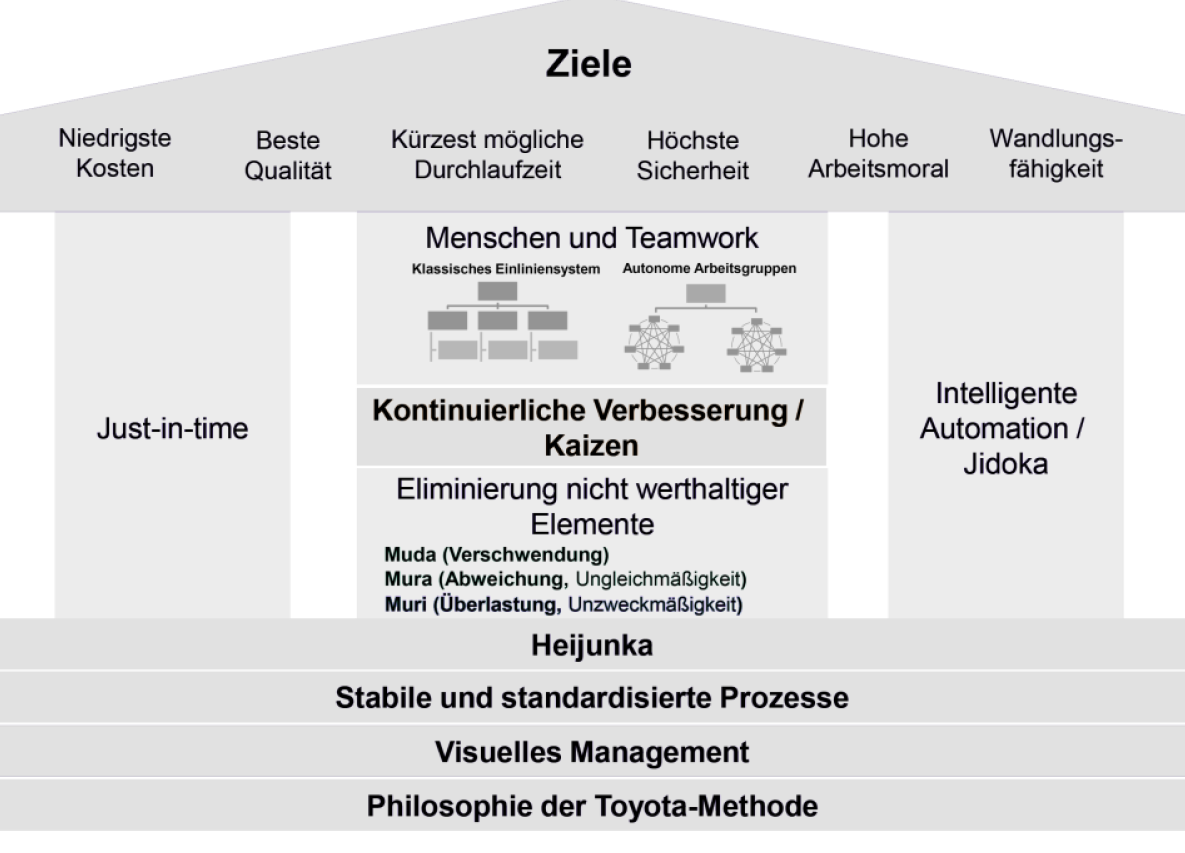
\includegraphics[width=0.7\textwidth]{TPS.png}
  \caption{Toyota Produktionssystem}
  \label{TPS}
\end{figure}

\clearpage

\section{Prinzipien}

Liker fand nun heraus, dass diese Prinzipien im gesamten Unternehmen angewendet werden und formulierte so den Toyota Weg. Dieser setzt sich aus den 14 Prinzipien zusammen die er in seinem Buch beschreibt. Dabei unterteilt er diese in 4 Kategorien. Diese 4 Kategorien können auch als 4 P's beschrieben werden. Zusammen bilden sie eine Pyramide wie in Abb. \ref{4P} zu sehen ist. An der Spitze steht die Problemlösung. Dabei finden das kaizen und genchi genbutsu Anwendung. Das sind japanische Begriffe die bei Toyota für die Beschreibung der Prinzipien genutzt werden. Das zweite P steht für Personen und Partner. Dabei hat Liker herausgefunden, dass Toyota nur bestimmte Führungskräfte einstellt und ihre Lieferanten mit Bedacht auswählt. Das dritte P ist der Prozess. Darin finden sich die meisten Prinzipien wieder. Das vierte P ist das wichtigste Prinzip. Auf der Philosophie beruhen alle Entscheidungen. Dabei geht es Toyota vorrangig um langfristiges Denken. Worauf die Philosophie und die anderen Prinzipien genauer abzielen, wird in den folgenden Kapiteln erklärt.

\begin{figure}[h] 
  \centering
     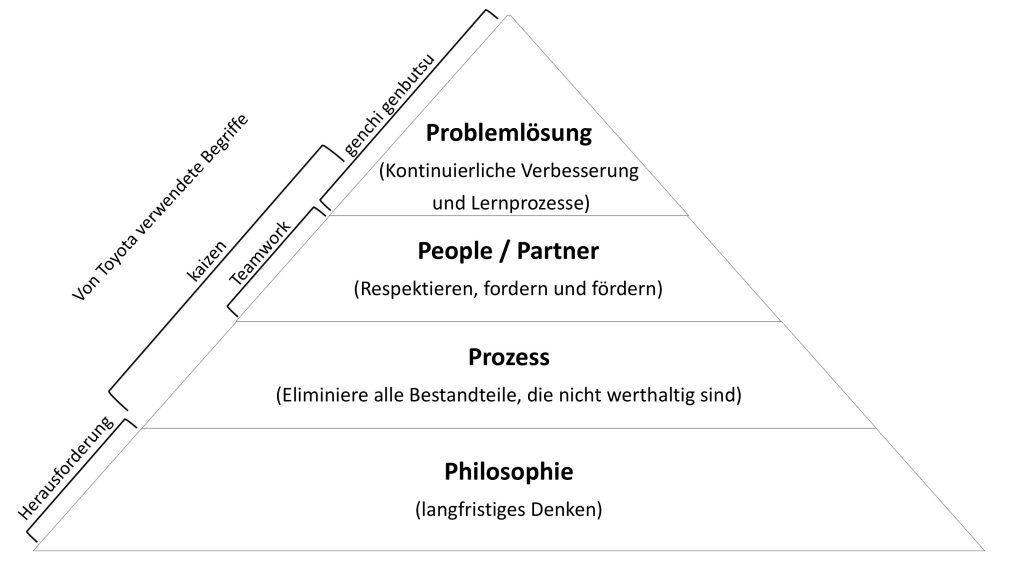
\includegraphics[width=0.7\textwidth]{4P.jpg}
  \caption{4P Modell des Toyota Weges}
  \label{4P}
\end{figure}

\subsection{Philosophie}



\subsubsection{1. Prinzip: Langfristiges Denken}

Toyotas Leitsatz bei der Philosophie lautet: "Machen Sie eine langfristige Philosophie zur Grundlage Ihrer Managemententscheidungen, selbst wenn diese zu Lasten kurzfristiger Gewinnziele geht". Ein gutes Beispiel dafür ist die Geschichte des Toyota Werkes in Long Beach Kalifornien. In den 60er Jahren erließen die USA Einfuhrzölle von 30\% auf Lastwagen. Da Toyota auch weiterhin Lastwagen in die USA exportieren wollte musste eine Lösung her. Andere Unternehmen fanden einen Weg und schickten den LKW ohne Ladefläche und die Ladefläche getrennt voneinander in die USA. Da diese als Komponenten zählten mussten dafür keine Zölle bezahlt werden. Toyota wandte den gleichen Trick an, stellte aber seine Ladeflächen direkt vor Ort her. Das ist nämlich eine der Philosophie Grundsätze, stärke die lokale Wirtschaft einer Region. Dieses Werk lief nun mehrere Jahrzehnte sehr gut. Kurz vor seinem 30 Jährigen Bestehen wollte man es schließen und nach Mexico outsourcen, da dort die Löhne billiger waren. Somit hätte Toyota ein kurzfristiger Gewinn erwartet, der aber zu Lasten der langfristigen Ziele genommen worden wäre. Man überwarf die Pläne und ist nun sehr stolz auf das Werk, welches nun Brennstoffzellen für LKW's herstellt.
Liker beschreibt in seinem Buch, dass die Philosophie Toyotas auf 3 wesentliche Punkte zielt. Zum einen die Wertgenerierung für den Kunden, die Gesellschaft und die Wirtschaft. Dabei findet er auch 7 Punkte die die Philosophie gut zusammenfassen:

\begin{itemize}
    \item Wir ehren die Sprache und den Geist der Gesetzgebung jedes Landes und achten auf offene und faire Unternehmensaktivitäten, um ein guter Bürger der Weltgemeinschaft zu sein.
    \item Wir respektieren die Sitten und Gebräuche jedes Landes und leisten durch Unternehmensaktivitäten in unserer jeweiligen Standortgemeinde einen Beitrag zur wirtschaftlichen und gesellschaftlichen Entwicklung.
    \item Wir bekennen uns zu umweltgerechten und sicheren Produkten und zur Verbesserung der Lebensqualität, und zwar an jedem Standort und in all unseren Aktivitäten.
    \item Wir erfinden und entwickeln fortgeschrittene Technologien und bieten herausragende Produkte und Dienstleistungen, die die Bedürfnisse unserer Kunden weltweit erfüllen.
    \item Wir fördern eine Unternehmenskultur, die die Kreativität jedes Einzelnen und den Wert der Teamarbeit steigert und gleichzeitig gegenseitiges Vertrauen und Respekt zwischen den Arbeitskräften und der Unternehmensführung schafft.
    \item Wir verfolgen Wachstum in Harmonie mit der globalen Gemeinschaft, und zwar durch innovatives Management.
    \item Wir arbeiten mit Geschäftspartnern in der Forschung und Entwicklung zusammen, um ein stabiles, langfristiges Wachstum und beiderseitigen Nutzen zu schaffen, während wir uns gleichzeitig offen halten für neue Partnerschaften.
\end{itemize}



\subsection{Prozesse}

Das zweite P was Liker in seinem Buch beschreibt ist der Prozess. Hier steht die Eliminierung von Verschwendungen, auch muda genannt, im Vordergrund. Instrumente die darauf aufbauen können sind zum Beispiel das Pull System oder die Möglichkeit nur zuverlässige Technologien einzusetzen. Diese Kategorie teilt sich in 7 Prinzipien welche nachfolgend genauer betrachtet werden. 

\subsubsection{2. Prinzip: One-Piece Flow}

Hauptaugenmerk beim One-Piece-Flow ist die Eliminierung von Verschwendungen. Dabei ist es wichtig herauszufinden was wertschöpfende Tätigkeiten sind und was nicht. So kann es auch mal sein, dass ein Prozess aus 90\% warten und 10\% wertschöpfender Tätigkeit besteht. Wenn man nun diese 90\% eliminieren kann, ist es möglich einen Prozess der über Tage ging auf wenige Stunden zu beschränken. Diese Verschwendungen können laut Liker folgende Punkte sein:

\begin{itemize}
    \item Überproduktion
    \item Wartezeiten
    \item unnötige Transporte
    \item zu viele oder falsche Prozessschritte
    \item Lagerüberhänge
    \item unnötige Bewegungen
    \item Fehler
    \item ungenutzte Kreativitätspotenziale der Mitarbeiter
\end{itemize}

Ist man nun in der Lage diese zu eliminieren wie es Toyota immer wieder schafft, kann man folgende Vorteile daraus ziehen:

\begin{itemize}
    \item Qualitätsverbesserung\\
    Es ist viel einfacher, in einem One-Piece-Flow eine hohe Qualität zu erzielen. Jeder Montagearbeiter bzw. Maschinenbediener fungiert als Inspektor und arbeitet daran, an seiner Arbeitsstation auftretende Probleme zu lösen, statt sie an die nächste Stufe der Weiterverarbeitung weiterzureichen. Falls Mängel an einer Arbeitsstation übersehen werden, dauert es aber nicht lange, bis sie entdeckt werden, so dass das Problem schnellstmöglich diagnostiziert und beseitigt werden kann.
    \item Echte Flexibilität\\
    Wenn Maschinen für eine bestimmte Fahrzeuglinie eingesetzt werden, lassen sie sich nicht mehr flexibel für andere Zwecke einsetzen. Wenn die Durchlaufzeiten zur Herstellung eines Produkts aber sehr kurz sind, würde genau dies eine größere Flexibilität in der Reaktion auf Kundenbedürfnisse schaffen. Statt ein System neu auszurichten und wochenlang darauf zu warten, bis das Produkt endlich fertig ist, können neue Aufträge bei kurzen Durchlaufzeiten innerhalb weniger Stunden erfüllt werden. Die Umrüstung auf einen anderen Produktmix als Anpassung an eine veränderte Kundennachfrage kann fast umgehend erfolgen.
    \item Produktivitätssteigerung\\
    Der Grund, warum die Produktivität höher zu sein scheint, wenn Ihr Betrieb in Fachabteilungen untergliedert ist, hängt damit zusammen, dass jede Abteilung an der Auslastung ihrer Maschinen und Mitarbeiter gemessen wird. Tatsächlich ist es bei der Batch-and-Queue-Methode aber sehr schwer zu bestimmen, wie viele Mitarbeiter wirklich benötigt werden, um eine bestimmte Zahl an Einheiten herzustellen, weil sich die Produktivität nicht nach der Wert schöpfenden Arbeit bemisst. Wer weiß, wie viel Produktivität dadurch verloren geht, dass Mitarbeiter damit „ausgelastet“ werden, Warenüberhänge zu produzieren, die dann in Lagern gestapelt werden müssen? Wie viel Zeit geht dadurch verloren, dass defekte Teile und Komponenten nachverfolgt und fertige Produkte nachgebessert werden müssen? In einer One-Piece-Flow-Zelle gibt es kaum nicht werthaltige Aktivitäten wie z.B. den Transport von Materialien von einer Arbeitsstation zur nächsten. Es wird sofort ersichtlich, wer überlastet und wer nicht ausgelastet ist. Es ist leicht, den Anteil der werthaltigen Arbeit zu berechnen und dann zu kalkulieren, wie viele Mitarbeiter benötigt werden, um eine bestimmte Produktionsquote zu erreichen. In jedem einzelnen Fall, in dem das Toyota Supplier Support Center die Massenproduktion der Zulieferer auf TPS umstellten, wurde ein Zuwachs an Arbeitsproduktivität von mindestens 100 Prozent erzielt.
    \item Reduzierung der benötigten Werksfläche\\
    Die Aufstellung der Maschinen nach Abteilungen schafft große ungenutzte Freiflächen zwischen den einzelnen Maschinen. Die größte Platzverschwendung entsteht jedoch durch Zwischenlager mit Stapeln an Teilen und Komponenten. In einer Zelle sind alle Prozessschritte nahe beieinander angeordnet, Zwischenlager gibt es kaum. Durch die bessere Ausnutzung der Werksfläche lässt sich die sonst unvermeidliche Aufstockung der Kapazitäten vermeiden.
    \item Erhöhung der Sicherheit\\
    Kleinere Teilemengen bedeuteten, dass man auf große Gabelstapler verzichten konnte, die häufig zu Unfällen führen. Es bedeutete auch, dass kleinere Materialcontainer gehoben und transportiert werden mussten. Unfälle im Zusammenhang mit dem Heben schwerer Gewichte würden sich also auch nicht mehr ereignen. Die Sicherheit stieg mit dem Fokus auf einen Prozessfluss – auch ohne einen speziellen Fokus auf das Thema Sicherheit.
    \item Steigerung der Arbeitsmoral\\
    In einem One-Piece-Flow verrichten die Mitarbeiter mehr werthaltige Arbeit und sehen unmittelbar die Ergebnisse ihrer Arbeit. Das vermittelt das Gefühl, etwas geleistet zu haben und schafft so Arbeitszufriedenheit.
    \item Reduzierung der Kosten für die Lagerhaltung\\
    Sie setzen auf diese Weise totes Kapital für andere Investitionen frei. Außerdem entfallen die Kosten der Lagerhaltung. Auch die Überalterung des Lagerbestands sinkt.
\end{itemize}

\subsubsection{3. Prinzip: Pull-System}

Das nächste Prinzip was Liker in die Kategorie Prozesse einordnet ist die Verwendung des Pull-Systems. Der Unterschied zwischen Pull und Push besteht in der Richtung der Lieferketten.Bei der Push Methode stellt der Zulieferer Teile her und schickt sie nach der Fertigung an Toyota. Diese können die Menge ab Teilen nicht direkt verarbeiten und lagern diese zwischen. Das dies zu Problemen vor allem in der Lagerhaltung führt liegt in der Hand. Toyota nutzt deswegen das Pull-System. Wobei sie bestimmen wann ein Teil geliefert werden soll. Somit fängt der Lieferant erst an das Teil zu produzieren sobald der Auftrag von Toyota eingegangen ist. Dieses Vorgehen vermeidet Lagerrückstände und benötigt ein dezentrales Steuerungssystem. Auch ein stetiger Materialfluss ist wichtig. Deswegen ordert Toyota nie mehr als es benötigt und kann somit seinen Just-in-Time Ansatz umsetzen. 

\subsubsection{4. Prinzip: Heijunka}

Das 4.Prinzip nennt sich Heijunka. Hierbei geht es Toyota um die Ausgeglichenheit des Arbeitsablaufes. Liker beschreibt dies mit den 3 M's, muda, mura und muri. Muda wurde bereits beschrieben. Muri bedeutet Überbelastung von Mensch und Maschine. Mura bedeutet Ungleichgewicht. Diese 3 dürfen nicht überhand gewinnen damit das System ausgeglichen bleiben kann. Ein wichtiger Punkt dabei ist es die Bestellungen nicht nach Ordereingang zu bearbeiten. Toyota betrachtet die Bestellungen über einen Zeitraum und passt dann die Herstellungsreihenfolge daraufhin an. Hauptaugenmerk dabei ist, dass Mensch und Maschine so wenig Belastung wie möglich aushalten müssen. Ein wichtiger Punkt dabei ist die Flexibilität. Vor allem die der Maschinen. So ist es Toyota gelungen die Wechselzeiten von Produktionsbändern so zu verkürzen, dass noch während des Betriebes ein Band von der Herstellung eines Produktes auf ein anderes umgestellt werden kann. Dies kann man sich wie ein Boxenstopp in der Formel 1 vorstellen. Somit wird das "build to order" ein "change to order".

\subsubsection{5. Prinzip: Jidoka}

Das 5.Prinzip heißt Jidoka und beschreibt die Kultur Toyotas auf Anhieb Qualität zu liefern und nicht ständige Verbesserungen ausführen zu müssen. Dabei wird meist der gesamte Prozess unterbrochen wenn ein Fehler auftritt um die Qualität auf Anhieb sicher zu stellen und nicht auf unnötige Nachbesserungen angewiesen zu sein. 4 Schritte kristallisiert Liker dabei heraus:

\begin{itemize}
    \item Mach dir selbst ein Bild
    \item Führe eine ausführliche Analyse durch
    \item Benutze das andon-Prinzip 
    \item Frage 5 mal Warum
\end{itemize}

Das andon Prinzip ist eine Möglichkeit die Fehler in der Produktion anzuzeigen. Also wie eine Alarmleuchte bei einer Produktionsanlage, die einen zeigt wo das Problem liegt.

\subsubsection{6. Prinzip: Standardisierung}

Das 6. Prinzip ist die Standardisierung der Arbeitsschritte. Das Ziel aller Produktionsschritte ist natürlich die Verbesserung der Produktion. Das kann man nur schaffen wenn die Prozesse einen Standardweg besitzen den die Mitarbeiter ausführen. Das ist das selbe wie beim Golf. Wenn man nicht einmal standardmäßig den Ball trifft, kann man auch nicht sein Golfschwung verbessern. 
Toyotas Weg zur Standisierung sieht wie folgt aus. Sie verscuhen jeden Mitarbeiter in die Bestimmung solcher Arbeitsstandards mit einzubeziehen. Dazu werden sogenannte Pilot Teams gebildet, deren Aufgabe es ist neue Standards festzulegen. So ein Pilot Team besteht aus Mitarbeitern aller Schichten und Abteilungen. Aller 3-4 Jahre wechselt die Belegung eines solchen Teams. Dadurch ist jeder in der Lage die Standards zu bestimmen und es kommt auch nicht zu Beschwerden wenn neue Standards eingeführt werden, da jede Abteilung Mitspracherecht hat. Somit ist Toyotas Weg hier präzise genug um solche Standards fest zulegen, lässt den Mitarbeitern aber auch genügend Freiraum zur kreativen Gestaltung.

\subsubsection{7. Prinzip: Visuelles Management}

Das visuelle Management beschreibt das 7.Prinzip des Toyota Weges. Dieses wird in die 5 S's eingeteilt:

\begin{enumerate}
    \item Seiri: Sortieren\\
    Sortieren Sie alle Dinge und behalten Sie nur das, was Sie wirklich brauchen, und entsorgen Sie alles andere.
    \item Seiton: Ordnungsliebe \\
    Ein Platz für alles und alles an seinen Platz.
    \item Seiso: Sauberkeit\\
    Beim Saubermachen findet meistens gleichzeitig eine Inspektion statt, bei der man auf Unregelmäßigkeiten und drohende Mängel aufmerksam wird, die zu Qualitätseinbußen oder Maschinenausfällen führen können.
    \item Seiketsu: Standardisieren/Regeln schaffen \\
    Entwickeln Sie Systeme und Verfahren, um die Einhaltung der ersten drei S zu überwachen.
    \item Shitsuke: Selbstdisziplin \\
    Die Beibehaltung eines stabilen Arbeitsablaufs ist ein kontinuierlicher Verbesserungsprozess. Disziplin ist natürlich der schwerste Prozess wie jeder selber weiß
\end{enumerate}

\subsubsection{8. Prinzip: Vetrauenswürdige Technologien}

Das letzte Prinzip der Kategorie Prozesse ist der Leitsatz, dass Toyota nur Technologien benutzt die zuverlässig sind. Es ist nämlich so dass sich Toyota sehr viele Gedanken macht bevor eine neue Technologie, wie eine neue Software eingeführt wird. Dazu hat Liker den Ablauf wie folgt beschrieben. Wenn eine neue Technologie auf den Markt kommt, beginnt Toyota mit einer umfassenden Analyse. Dabei bilden sie eine pilot area in der Abteilung wo die neue Technologie eingeführt werden könnte. In dieser pilot area wird aber nicht die Technologie getestet, sondern erstmal alle anderen Instrumente und Werkzeuge zur Produktivitätssteigerung angewendet die Toyota bis dahin zur Verfügung stehen. Sollten durch die Methoden keine Verbesserungen erzielt werden, kann man genauer über die Einführung der Technologie nachdenken. Dabei muss diese aber mit den vorangegangenen Prinzipien übereinstimmen. Diese Technologie sollte den Menschen über die Maschine stellen, das Konsensprinzip wahren, Verschwendung vermeiden, flexibel, visuell und intuitiv sein. Bei dieser Entscheidung sind alle Beteiligten des Prozesses involviert. Der Entscheider ist dann der Ingenieur vor Ort der die neue Technologie betreuen wird. 

\subsection{Personen und Partner}

Die 3. Kategorie die Liker in seinem Buch beschreibt nennt er Personen und Partner. Dabei geht es Toyota vor allem um die Team- und Netzwerkbildung sowie um die Führungskräfte. Wie Toyota diese auswählt und was diese auszeichnet wird folgend beschrieben. 

\subsubsection{9. Prinzip: Führungskräfte}

Das wichtigste für die Führungskräfte ist dass sie die Firmenphilosophie verinnerlicht haben und diese anderen vorleben und vermitteln. Dabei achtet Toyota darauf dass diese intern ausgebildet werden anstatt einen neuen Mitarbeiter zu rekrutieren. Ein wichtiger Bestandteil der Toyota Führungskräfte ist der Chefingenieur. Dieser bildet die Schnittstelle zwischen Abteilung und Produktionslinie. Als kritische Schnittstelle zwischen Innovationen, Führungsebene und Kundenzufriedenheit haben sie die Rückendeckung des Topmanagements. Der Chefingenieur hat das Ohr der Führungsspitze, die sich dazu verpflichtet ihm alle für den Erfolg nötigen Ressourcen zur Verfügung zu stellen. 
Bei der Beobachtung vieler Manager hat Liker herausgefunden dass fast alle diese Gemeinsamkeiten haben:

\begin{itemize}
    \item Fokussierung auf das langfristige Ziel
    \item Keinerlei Abweichen vom Kern der Toyota DNA
    \item Hocharbeitung im Unternehmen selbst
    \item Betrachtung von Problemen als Chance, die Mitarbeiter zu schulen und weiterzuentwickeln
\end{itemize}

\subsubsection{10. Prinzip: Team}

Das 10. Prinzip beinhaltet das Team. Dazu beschreibt Liker die Herangehensweise von Blanchard aus dem Buch "One Minute Manager". Dieser teilt die Teambildung in 4 Stationen ein:

\begin{enumerate}
    \item Stufe: Orientierung \\
    Die Gruppe braucht eine starke Führung von einem Gruppenleiter und muss die grundlegende Mission, die Regeln für Engagement und die Instrumente erlernen, die die Gruppenmitglieder anwenden.
    \item Stufe: Unzufriedenheit \\
    Die Gruppe macht sich an die Arbeit. Das ist nur halb so unterhaltsam wie die Gespräche über die großen Erfolgsvisionen, und die Gruppenmitglieder erkennen, dass die Arbeit in einer Gruppe anstrengender ist, als sie erwartet haben. In diesem Stadium brauchen sie sowohl die starke Führung (Struktur) eines Gruppenleiters als auch viel zwischenmenschliche Unterstützung, um durch die harten gruppendynamischen Prozesse zu gehen, die sie nicht verstehen.
    \item Stufe: Integration \\
    Die Gruppe gewinnt allmählich ein klareres Bild von der Rolle der verschiedenen Gruppenmitglieder und beginnt, Kontrolle über die Gruppenprozesse auszuüben. Die Herausforderung an die Gruppe besteht darin, Rollen, Ziele, Normen und die Gruppenstruktur zu erkennen. Der Gruppenleiter muss nicht mehr so viel Unterstützung hinsichtlich der konkreten Aufgabenstellung, aber noch sehr viel soziale Unterstützung leisten.
    \item Stufe: Produktion\\
    Die Gruppe hat ihre Lektionen aus den ersten drei Stufen gelernt und funktioniert nun als Hochleistungsteam und kommt weitgehend ohne die operative oder soziale Unterstützung des Gruppenleiters aus.
\end{enumerate}

Laut Blanchard können diese Stufen in mehreren Meetings erreicht werden. Bei Toyota ist es aber so, dass sie den Ansatz verfolgen, dass sich Teams nur während der eigentlichen Arbeit bilden. Somit kann ein Teamaufbauprozess auch mal mehrere Jahre dauern. Dabei erkennt man auch wieder das Zusammenspiel aller Prinzipien und Instrumente. Nämlich wenn man den One-piece-Flow eingeführt hat, müssen alle Mitarbeiter eng zusammen arbeiten und sich gegenseitig unterstützen. Das formt eine Gruppe natürlich zu einem Team, da diese die Arbeit nur gemeinsam gut erledigen können.

Ein typisches Toyota Organigramm sieht wie folgt aus:

\begin{itemize}
    \item Teammitglieder
    \begin{itemize}
        \item führen Arbeit nach aktuellem Standard aus
        \item befolgen 5 S in ihrem Arbeitsbereich
        \item führen kleinere Routinewartungsarbeiten durch
        \item suchen nach Verbesserungsmöglichkeiten
        \item unterstützen kleinere Gruppenaktivitäten bei der Problemlösung
    \end{itemize}
    \item Teamleiter
        \begin{itemize}
        \item initiieren Prozess-Startup und -kontrolle
        \item sorgen für die Einhaltung der Produktionsziele
        \item reagieren auf andon-Rufe der Teammitglieder
        \item führen Routinequalitätschecks durch
        \item springen für abwesende Teammitglieder ein
        \item führen Schulungen durch
        \item erteilen Arbeitsanweisungen
        \item stellen sicher, dass Standardverfahren eingehalten werden
        \item fördern Gruppenaktivitäten
        \item sorgen für ständige Projekte der kontinuierlichen Verbesserung
        \item sorgen für einen reibungslosen Nachschub an Material und Teilen
    \end{itemize}
    \item Gruppenleiter
        \begin{itemize}
        \item machen die Urlaubs- und Einsatzplanung
        \item sind für monatliche Produktionsplanung verantwortlich
        \item übernehmen administrative Aufgaben
        \item achten auf die Wahrung der Teammoral
        \item bestätigen Routinequalität und Qualitätschecks der Teamleiter
        \item koordinieren die Schichtübergänge
        \item führen Prozesstests und -veränderungen durch
        \item sorgen für die Entwicklung der Teammitglieder und funktionsübergreifende Trainings
        \item berichten über die täglichen Produktionsergebnisse
        \item realisieren Kosteneinsparungen
        \item führen Projekte zur Prozessverbesserung, Produktivität, Qualität und Ergonomie durch
        \item koordinieren umfangreiche Wartungsarbeiten
        \item koordinieren Unterstützung durch externe Gruppen
        \item koordinieren die Arbeit mit vor- und nachgelagerten Prozessen
        \item sorgen für die Einhaltung der Standards und Sicherheit der Gruppe
        \item springen für abwesende Teamleiter ein
        \item koordinieren die Aktivitäten rund um die Umrüstung auf andere Fahrzeugmodelle
    \end{itemize}
\end{itemize}

Dabei kann man erkennen, dass die Verantwortung und die Aufgaben immer mehr werden, je höher man kommt. 

\subsubsection{11. Prinzip: Netzwerk}

Das 11.Prinzip besagt, dass man ein hervorragendes Netzwerk an Geschäftspartnern braucht. Toyota verfolgt den Ansatz dass sie diese fördern und fordern. Dabei sind die Zulieferer für das Just-in-Time Verfahren sehr wichtig. Denn wenn man sich auf diese nicht verlassen kann, bricht die gesamte Produktionskette ein. Toyota vertraut dabei auf langjäghrige Geschäftspartner und verfolgt den Ansatz dass man gemeinsam wachsen sollte. Wenn man neue Zulieferer sucht, bekommen diese erst einmal nur kleine Aufträge um sich das Vertrauen von Toyota zu erarbeiten. Dazu müssen diese den hohen Anforderungen von Toyota gerecht werden. Liker beschreibt den Weg den Toyota mit seinen Partnern einschlägt über die Pyramide in Abb. \ref{Netzwerk}. Das große Ziel dabei ist es ein lernendes Unternehmen als Partner zu etablieren. Dabei geht es über die Schritte der fairen Beziehungen, klaren Erwartungen und stabien Prozessen.

\begin{figure}[h] 
  \centering
     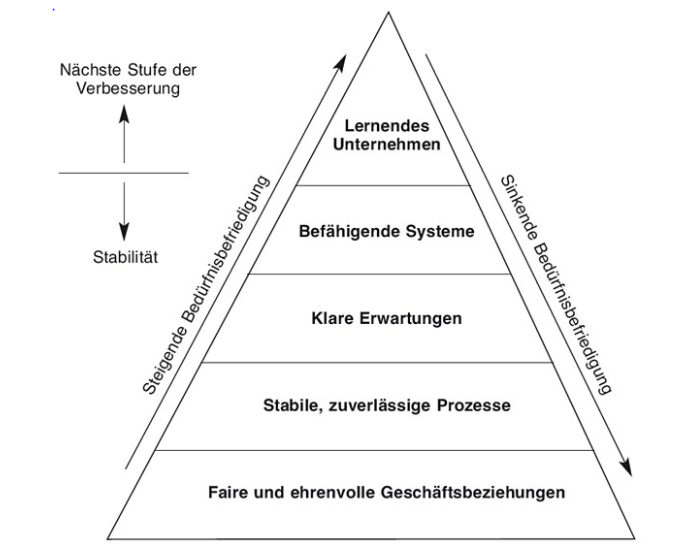
\includegraphics[width=0.6\textwidth]{Netzwerk.png}
  \caption{Bedürfnishierarchie der Zulieferkette}
  \label{Netzwerk}
\end{figure}


\subsection{Problemlösung}

Die letzte Kategorie ist die Problemlösung. Dabei ist Toyotas größtes Ziel ein lernendes Unternehmen zu werden. Die einzelnen Prinzipien die Toyota dabei helfen werden nachfolgend beschrieben.

\subsubsection{12. Prinzip: Genchi Genbutsu}

Genchi Genbutsu sagt aus, dass man sich selbst ein Bild vor Ort machen sollte, um das Problem umfassend zu verstehen. Ein gutes und berühmtes Beispiel ist der Ohno Kreis. Ohno war der Werksleiter der das Toyota Produktionssystem entwickelt hat. Dabei gab er seinen Mitarbeitern die Aufgabe einen Kreis auf dem Boden zu zeichnen um sich einen Tag lang hinein zu stellen und die Prozesse aus nächster Nähe zu betrachten. Dadurch bekamen sie ein sehr gutes Bild davon was schief läuft. Liker beschreibt die Herangehensweise bei der Beobachtung von Toyota wie folgt:

\begin{itemize}
    \item Behalten Sie immer das Endziel im Kopf
    \item Planen Sie sorgfältig auf Ihr Endziel hin
    \item Sorgen Sie dafür, dass Meetings einem eindeutigen Zweck dienen
    \item Übertragen Sie sich selbst und anderen klare Aufgaben
    \item Denken und sprechen Sie auf Basis verifizierter, verlässlicher Informationen und Daten
    \item Vergewissern Sie sich persönlich von der Richtigkeit der Fakten
    \item Sie sind verantwortlich für die Informationen, die Sie anderen geben
    \item Teilen Sie Ihre Informationen zeitnah mit anderen
    \item Denken Sie immer daran wer von diesen Informationen profitieren wird
    \item Verstehen Sie Ihre Defizite und Kompetenzen auf eine messbare Art und Weise
    \item Klären Sie welches Wissen Sie brauchen um sich selbst weiterzuentwickeln
    \item Streben Sie unermüdlich danach kaizen-Maßnahmen durchzuführen
    \item Denken Sie über den Tellerrand hinaus
    \item Achten Sie stets darauf Ihre Sicherheit und Gesundheit zu schützen
\end{itemize}

\subsubsection{13. Prinzip: Nemawashi}

Das 13. Prinzip lautet Nemawashi. Das hat den Grundsatz, dass sie Entscheidungen mit Bedacht und nach dem Konsensprizip treffen sollten. Man sollte alle Alternativen sorgfältig abwägen, aber die getroffene Entscheidung zügig umsetzen. Bei der Entscheidungsfindung geht man ursprünglicherweise von 5 Schritten aus:

\begin{enumerate}
    \item Feststellung der aktuellen Situation
    \item Kennen und Verstehen der aktuellen Faktoren
    \item Prüfung einer breiten Palette an Alternativen
    \item Konsensbildung im Team
    \item Nutzung hocheffizienter Kommunikationsinstrumente
\end{enumerate}

Laut Liker beschreitet Toyota auch hier wieder einen alternativen Weg. Dieser ist in Abb. \ref{Entscheidung} zu sehen.


\begin{figure}[h] 
  \centering
     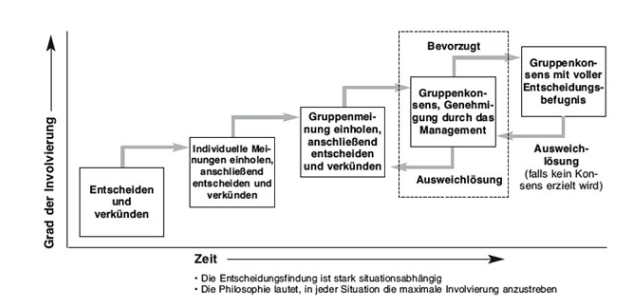
\includegraphics[width=0.7\textwidth]{Entscheidung.png}
  \caption{Toyotas Weg zur Entscheidungsfindung}
  \label{Entscheidung}
\end{figure}

Meetings sind auch ein wichtiges Instrument zur Entscheidungsfindung. Natürlich hat Toyota dafür auch einige Regeln aufgestellt:

\begin{enumerate}
    \item Klare Zielsetzung vor dem Meeting. Diese Ziele können sich in der Agenda wiederfinden, aber die Agenda muss sehr auf klar definierte Aufgaben und Ergebnisse fokussiert sein.
    \item Es müssen die richtigen Zielgruppen teilnehmen. Die Leute, die auf dem Meeting gebraucht werden, müssen auch erscheinen.
    \item Vorbereitete Teilnehmer. Alle Teilnehmer wissen, worauf sie sich für das Meeting vorbereiten müssen und haben ihre Hausaufgaben gemacht.
    \item Effektiver Einsatz visueller Verstärker. Das A3-Format ist äußerst effektiv.
    \item Trennung von Informationsaustausch und Problemlösung. Vor dem Meeting muss ein möglichst reger Informationsaustausch stattfinden, damit sich die Teilnehmer während des Meetings auf die Problemlösung konzentrieren können.
    \item Das Meeting beginnt und endet pünktlich.
\end{enumerate}

Dadurch erreicht Toyota eine außerordentliche Sammlung von Informationen die zur Entscheidungsfindung beitragen. Die Vorteile die sich daraus ergeben liegen auf der Hand. zum einen deckt es alle Fakten auf, deren Missachtung in einer späteren Phase des Entscheidungsprozesses viel Mühe machen und zu einer Neuaufwicklung bestimmter Schritte führen. Zudem geschieht die Ausführung meist fehlerfrei. Toyota bindet alle Betroffenen ein und gewinnt deren Unterstützung der Entscheidung, so dass mögliche Widerstände vor der Umsetzung ausgeräumt werden können. Die Kosten der Überwindung von Widerständen in der Umsetzungsphase wären aller Wahrscheinlichkeit nach wesentlich höher als in der Planungsphase. Toyota vollzieht noch vor der eigentlichen Planung und Umsetzung einen Lernprozess.

\subsubsection{14. Prinzip: Kaizen und Hansei}

Das letzte Prinzip nennt sich kaizen und hansei. Diese Begriffe bedeuten dass man sich durch unermüdliche Reflexion (hansei) und kontinuierliche Verbesserung(kaizen) zu einer wahrhaft lernenden Organisation entwickeln soll. Hansei ist dabei eine kulturelle Sache, die in Japan oft angewendet wird. Dabei setzt man sich kritisch mit der eigenen Leistung auseinander. Dafür hält Toyota Reflexionsmeetings ab, bei der der Mitarbeiter mit seiner Führungskraft über seine eigene Leistung spricht. Kaizen beschreibt die kontinuierliche Verbesserung, dabei benutzt Toyota das Schema aus Abb. \ref{Problem} um seine Probleme zu lösen. 

\begin{figure}[h] 
  \centering
     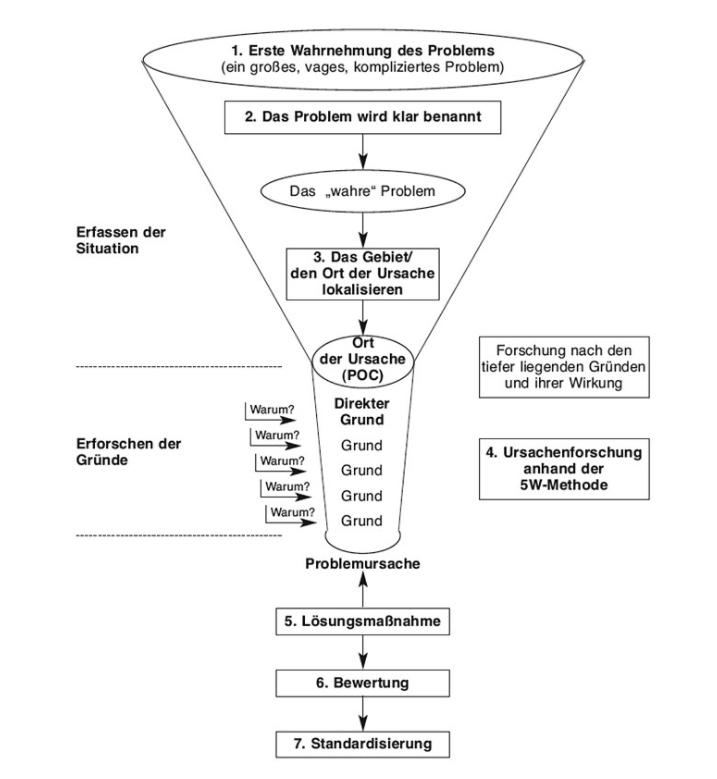
\includegraphics[width=0.7\textwidth]{Problem.png}
  \caption{Toyotas praktischer Problemlösungsprozess}
  \label{Problem}
\end{figure}

Die 7 Schritte sollen für eine langfristige Abstellung des Problems sorgen. Um die Verbesserungen im Unternehmen zu messen beschreibt Liker 3 Messgrößen die Toyota betrachtet:

\begin{enumerate}
    \item Globale Performance
    \item Operative Performance
    \item Anspruchsvolle Verbesserungsziele
\end{enumerate}

All diese Dinge führen nun dazu einen Flow zu kreieren, der es Toyota ermöglicht ein lernendes Unternehmen zu werden. Dabei werden immer wieder, die Probleme aufgedeckt, gelöst, bewertet und in den Arbeitsflow integriert.

\clearpage
  
\section{Fazit}

Das Zusammenspiel all dieser Prinzipien und Werkzeuge macht Toyota zu dem erfolgreichsten Automobilhersteller der Welt. Dabei geht es nicht um die einzelnen Verbesserungen sondern um die Mentalität der ständigen Verbesserung und des Zusammenspiels aller Punkte und Mitarbeiter. Toyota sieht nämlich den Respekt vor dem Menschen als wichtigsten Punkt seiner Agenda. Ich finde dass durch das Zusammenspiel der Prinzipien und den ganzheitlichen Ansatz Toyotas eine Atmosphäre geschaffen wird, die genügend Struktur für Produktivität gibt, aber auch genügend Freiraum gelassen wird zur kreativen Weiterentwicklung. 

\clearpage
\addcontentsline{toc}{section}{Literatur}
\begin{thebibliography}{99}

% For books
\bibitem{toyota_book} Jeffrey K. Liker \emph{Der Toyota Weg; 14 Managementprinzipien des weltweit erfolgreichsten Automobilkonzerns}, 8. Aufl. Finanzbuchverlag, München, 2013.


\bibitem{Abbildung 1} Abb. \ref{TPS}: Toyota Produktionssystem \url{https://d2ah727fsr7un8.cloudfront.net/users/154791/154791_FeYuSaDuwoXeyohu9422637115171218.png}, [Online Stand 24.09.2021].

\bibitem{Abbildung 2} Abb. \ref{4P}: 4P Modell des Toyota Weges \url{https://andreasgoetzer.de/wp-content/uploads/Jeffrey-Liker-4P-Modell-TPS-Toyota-Produktionssystem-e1514626930508.jpg}, [Online Stand 24.09.2021].

\end{thebibliography}
\end{document}

